% Integration snippet for IEEE Access paper materials.
% Paste these inputs into the manuscript body in the order that fits the final narrative.

% Dataset and configuration tables.
\begin{table}[t]
\centering
\caption{Public benchmark datasets used in the IEEE Access experiments.}
\label{tab:datasets}
\begin{tabular}{r l r r r l}
        \hline
        Task ID & Dataset & Instances & Features & Classes & Notes \\
        \hline
        31 & credit-g & 1000 & 61 & 2 & From result metadata \\
        37 & diabetes & 768 & 8 & 2 & From result metadata \\
        9946 & wdbc & 569 & 30 & 2 & From result metadata \\
        10093 & banknote-authentication & 1372 & 4 & 2 & From result metadata \\
        10101 & blood-transfusion-service-center & 748 & 4 & 2 & From result metadata \\
        \hline
\end{tabular}
\end{table}

\begin{table}[t]
\centering
\caption{Experimental configuration for the public-data IEEE Access artifact runs.}
\label{tab:experimental_configuration}
\begin{tabular}{l l}
        \hline
        Setting & Value \\
        \hline
        Datasets & 5 public benchmark datasets \\
        Seeds & 0--9 \\
        n\_explain & 50 \\
        posterior\_samples & 500 \\
        bootstrap\_samples & 50 \\
        top\_k & 5 \\
        lambda\_hyb & 0.5 \\
        train\_fractions & \{0.10, 0.25, 0.50, 0.75, 1.00\} \\
        max\_train\_rows & 2000 \\
        max\_test\_rows & 500 \\
        model & auto \\
        main output directory & results\_ieee \\
        sensitivity output directory & results\_ieee\_sensitivity \\
        \hline
\end{tabular}
\end{table}


% Main results narrative and supporting tables.
\section{Results}

\subsection{Public-Data Empirical Reference Coverage}

Table~\ref{tab:uncertainty_validation} summarizes the uncertainty-validation results across the five public benchmark datasets in Table~\ref{tab:datasets}. Bayesian-FPDE achieved high empirical reference coverage on average, with mean empirical\_reference\_coverage\_95 of 0.945 against leave-one-seed empirical references. Bootstrap-FPDE produced a similar mean empirical\_reference\_coverage\_95 of 0.944. These values should be interpreted only as coverage against the empirical reference used in the experiment; the public benchmark datasets do not provide ground-truth feature attributions, so these results do not measure true attribution coverage or known-truth calibration.

Per-dataset results in Table~\ref{tab:per_dataset_coverage} show that empirical reference coverage varied across datasets. The corresponding coverage and error-correlation behavior is visualized in Fig.~\ref{fig:public_uncertainty_empirical_reference_coverage} and Fig.~\ref{fig:public_uncertainty_error_correlation}. Bayesian-FPDE had a mean interval width of 0.120 and a mean posterior standard deviation of 0.031, giving uncertainty estimates that are comparable in scale to the bootstrap reference while retaining the Bayesian posterior summary.

\subsection{Stability Across Random Seeds}

Table~\ref{tab:stability} reports seed-to-seed stability metrics. Bayesian-FPDE produced relatively stable feature rankings across seeds, with mean Spearman correlation of 0.900, mean Pearson correlation of 0.961, mean top-k Jaccard overlap of 0.896, and mean sign agreement of 0.876. The boxplots in Fig.~\ref{fig:stability_spearman_boxplot} and Fig.~\ref{fig:stability_topk_jaccard_boxplot} provide the corresponding distributional view across public datasets.

These stability results indicate that the uncertainty-aware Bayesian-FPDE procedure preserved consistent feature-ranking behavior under random-seed variation in this benchmark setting. They should not be read as evidence of ground-truth attribution accuracy, because the experiment compares repeated empirical estimates rather than known true explanations.

\subsection{Training-Size Uncertainty Behavior}

Table~\ref{tab:training_size} shows how Bayesian-FPDE uncertainty changed as the training fraction increased from 0.10 to 1.00. Mean posterior standard deviation decreased from 0.0949 at the 0.10 training fraction to 0.0308 at the full-training setting, and mean credible interval width decreased from 0.3696 to 0.1197. At the same time, attribution\_distance\_to\_full\_train decreased from 0.0525 to 0.0000, while top-k Jaccard overlap with the full-training empirical reference increased from 0.769 to 1.000.

These trends, also shown in Fig.~\ref{fig:ci_width_vs_training_size} and Fig.~\ref{fig:distance_to_full_train_vs_training_size}, are consistent with narrower uncertainty intervals and smaller distances to the full-training empirical reference as more training data are used. The distance metric is a distance to the full-training empirical reference constructed in the experiment, not a distance to a true attribution.

\subsection{Baseline-Dependent Faithfulness Evidence}

Table~\ref{tab:faithfulness} reports baseline-dependent Faithfulness metrics. Bayesian-FPDE obtained a faithfulness correlation of 0.334, deletion AUC of 0.675, insertion AUC of 0.844, and combined score of 0.531. SHAP obtained the largest combined score in this aggregate table, while LIME and Bootstrap-FPDE were close to Bayesian-FPDE on the displayed combined score.

These Faithfulness metrics are best treated as complementary model-output consistency evidence. They depend on the perturbation baseline and evaluation protocol, and they should not be interpreted as proof that Bayesian-FPDE outperforms SHAP or LIME. The deletion and insertion examples in Fig.~\ref{fig:deletion_curves_examples} and Fig.~\ref{fig:insertion_curves_examples} provide qualitative context for the aggregate Faithfulness results.

\begin{table*}[t]
\centering
\caption{Uncertainty validation against leave-one-seed empirical references.}
\label{tab:uncertainty_validation}
\begin{tabular}{l r r r r r}
        \hline
        Method & empirical\_reference\_coverage\_95 & uncertainty-error corr. & CI width-error corr. & Mean CI width & Mean posterior std. \\
        \hline
        Bayesian-FPDE & 0.945 & -0.198 & -0.193 & 0.120 & 0.031 \\
        Bootstrap-FPDE & 0.944 & -0.157 & -0.139 & 0.107 & 0.030 \\
        \hline
\end{tabular}
\end{table*}

\begin{table*}[t]
\centering
\caption{Per-dataset empirical reference coverage; these values are not true attribution coverage.}
\label{tab:per_dataset_coverage}
\begin{tabular}{l r r r r}
        \hline
        Dataset & Bayesian-FPDE coverage & Bootstrap-FPDE coverage & Bayesian-FPDE mean CI width & Bayesian-FPDE posterior std. \\
        \hline
        credit-g & 0.995 & 0.989 & 0.034 & 0.009 \\
        diabetes & 1.000 & 1.000 & 0.148 & 0.038 \\
        wdbc & 0.980 & 0.980 & 0.123 & 0.032 \\
        banknote-authentication & 0.750 & 0.750 & 0.107 & 0.027 \\
        blood-transfusion-service-center & 1.000 & 1.000 & 0.186 & 0.048 \\
        \hline
\end{tabular}
\end{table*}

\begin{table}[t]
\centering
\caption{Stability of feature rankings and signs across random seeds.}
\label{tab:stability}
\begin{tabular}{l r r r r}
        \hline
        Method & Spearman & Pearson & Top-k Jaccard & Sign agreement \\
        \hline
        Bayesian-FPDE & 0.900 & 0.961 & 0.896 & 0.876 \\
        Bootstrap-FPDE & 0.901 & 0.960 & 0.896 & 0.878 \\
        Hyb-FPDE & 0.915 & 0.961 & 0.896 & 0.880 \\
        SHAP & 0.940 & 0.974 & 0.908 & 0.890 \\
        LIME & 0.861 & 0.813 & 0.951 & 0.761 \\
        \hline
\end{tabular}
\end{table}

\begin{table}[t]
\centering
\caption{Bayesian-FPDE uncertainty behavior across training fractions.}
\label{tab:training_size}
\begin{tabular}{r r r r r}
        \hline
        Train fraction & Mean posterior std. & Mean CI width & Distance to full-train ref. & Top-k Jaccard to full train \\
        \hline
        0.10 & 0.0949 & 0.3696 & 0.0525 & 0.769 \\
        0.25 & 0.0607 & 0.2358 & 0.0309 & 0.836 \\
        0.50 & 0.0434 & 0.1688 & 0.0191 & 0.879 \\
        0.75 & 0.0357 & 0.1386 & 0.0109 & 0.940 \\
        1.00 & 0.0308 & 0.1197 & 0.0000 & 1.000 \\
        \hline
\end{tabular}
\end{table}

\begin{table}[t]
\centering
\caption{Faithfulness metrics are baseline-dependent and are used as complementary model-output consistency evidence.}
\label{tab:faithfulness}
\begin{tabular}{l r r r r}
        \hline
        Method & Faithfulness corr. & Deletion AUC & Insertion AUC & Combined score \\
        \hline
        Bayesian-FPDE & 0.334 & 0.675 & 0.844 & 0.531 \\
        Bootstrap-FPDE & 0.306 & 0.675 & 0.844 & 0.532 \\
        Hyb-FPDE & 0.374 & 0.674 & 0.846 & 0.533 \\
        SHAP & 0.516 & 0.634 & 0.863 & 0.561 \\
        LIME & 0.422 & 0.670 & 0.840 & 0.532 \\
        \hline
\end{tabular}
\end{table}


% Main result figures referenced by the results section.
\begin{figure}[t]
\centering
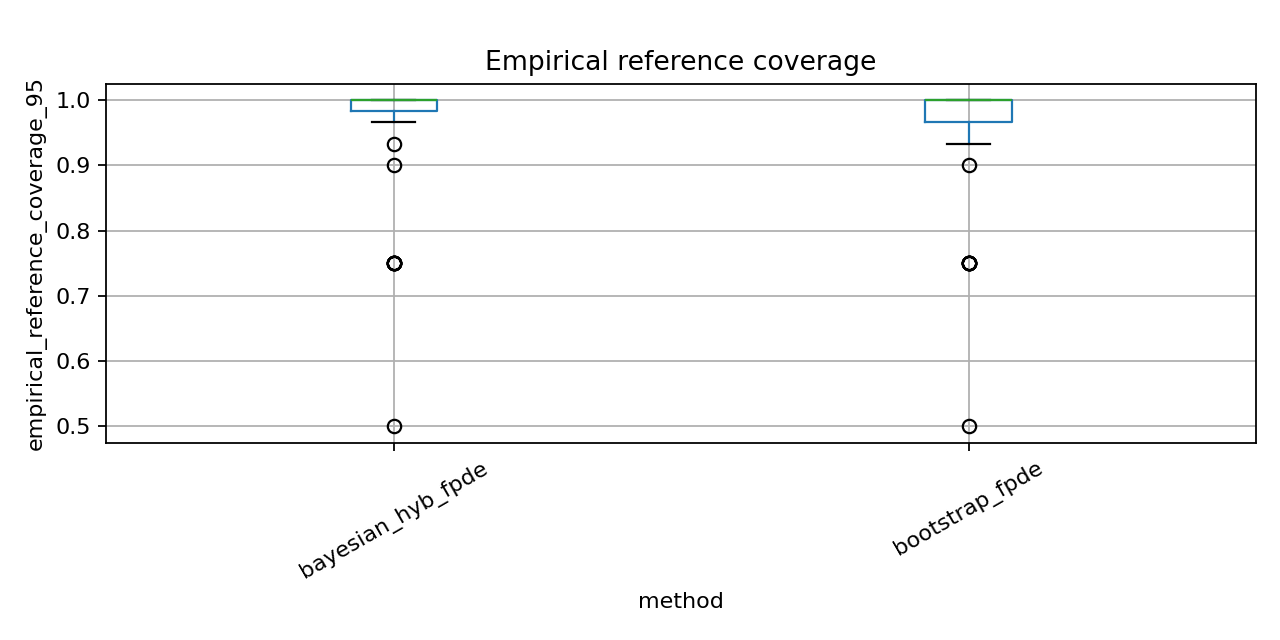
\includegraphics[width=\linewidth]{paper/figures/public_uncertainty_empirical_reference_coverage.png}
\caption{Empirical reference coverage against leave-one-seed empirical references.}
\label{fig:public_uncertainty_empirical_reference_coverage}
\end{figure}

\begin{figure}[t]
\centering
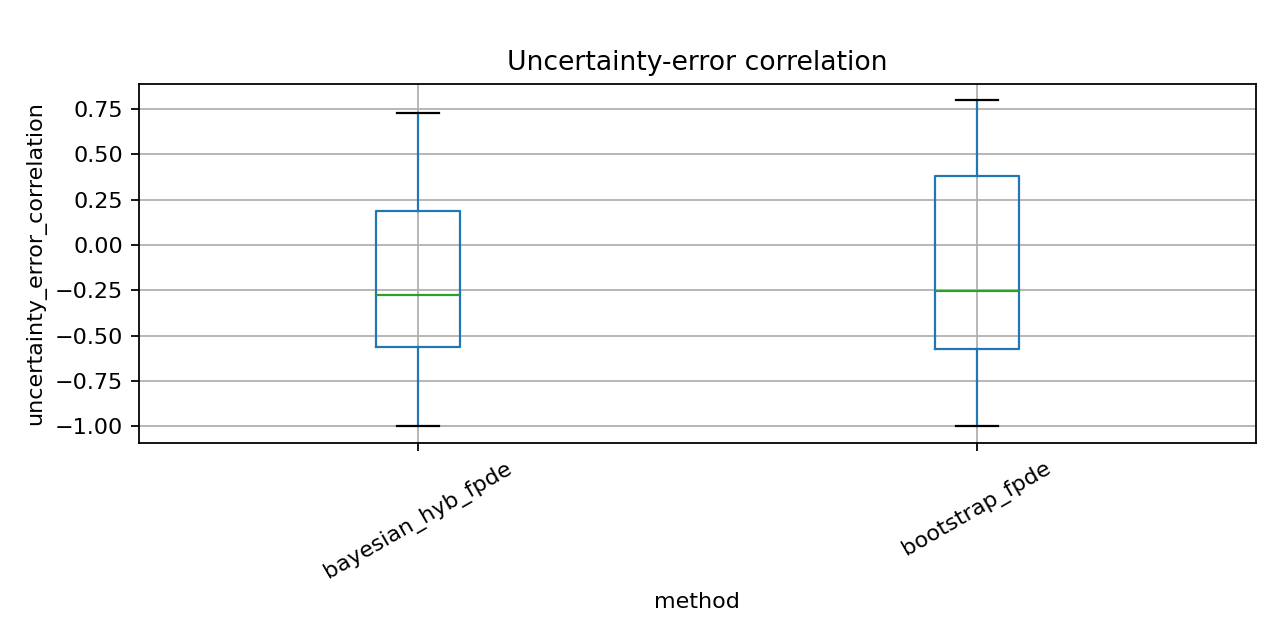
\includegraphics[width=\linewidth]{paper/figures/public_uncertainty_error_correlation.png}
\caption{Correlation between uncertainty summaries and error relative to leave-one-seed empirical references.}
\label{fig:public_uncertainty_error_correlation}
\end{figure}

\begin{figure}[t]
\centering
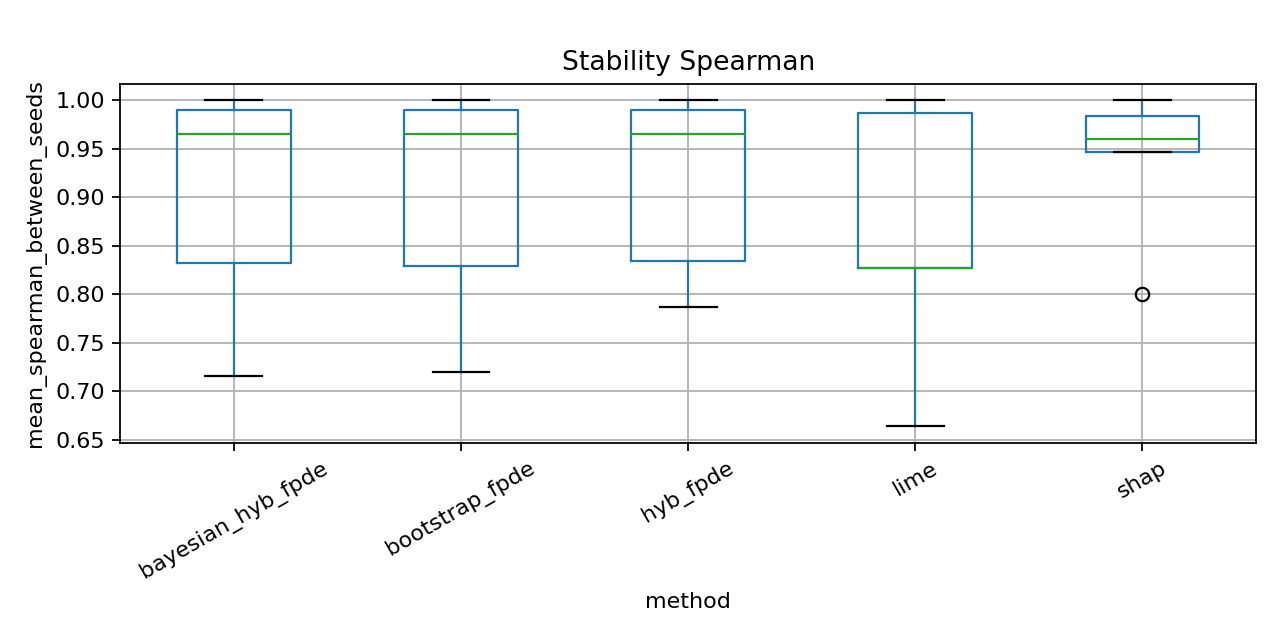
\includegraphics[width=\linewidth]{paper/figures/stability_spearman_boxplot.png}
\caption{Seed-to-seed Spearman rank stability of feature attributions across public benchmark datasets.}
\label{fig:stability_spearman_boxplot}
\end{figure}

\begin{figure}[t]
\centering
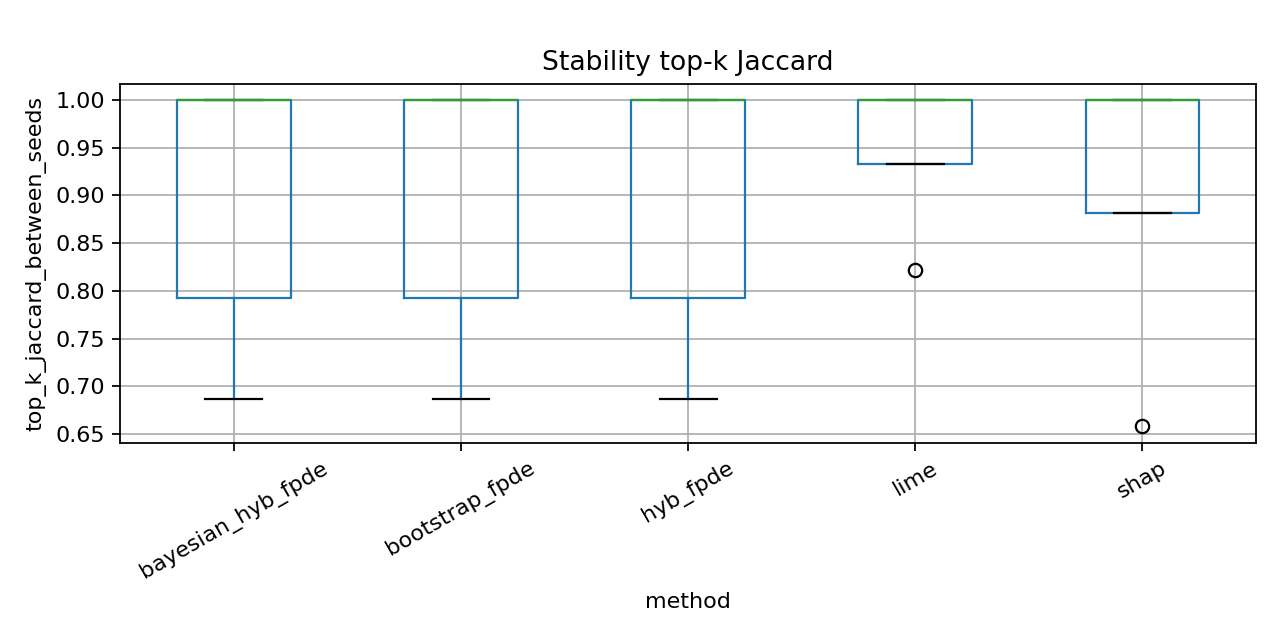
\includegraphics[width=\linewidth]{paper/figures/stability_topk_jaccard_boxplot.png}
\caption{Seed-to-seed top-k Jaccard overlap of feature rankings across public benchmark datasets.}
\label{fig:stability_topk_jaccard_boxplot}
\end{figure}

\begin{figure}[t]
\centering
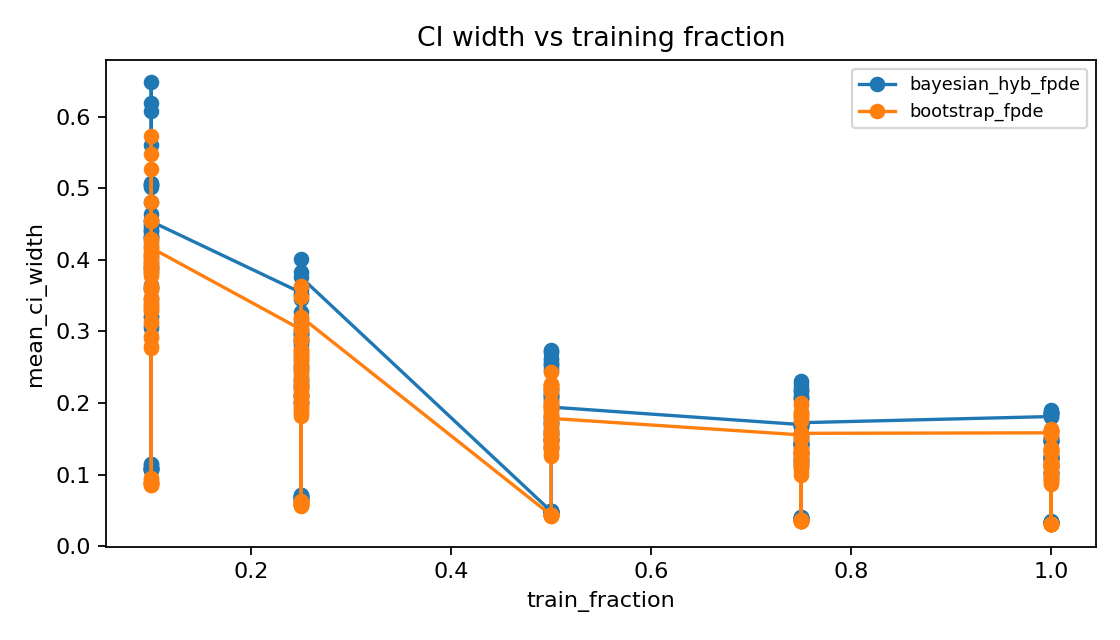
\includegraphics[width=\linewidth]{paper/figures/ci_width_vs_training_size.png}
\caption{Credible interval width as a function of training fraction for Bayesian-FPDE.}
\label{fig:ci_width_vs_training_size}
\end{figure}

\begin{figure}[t]
\centering
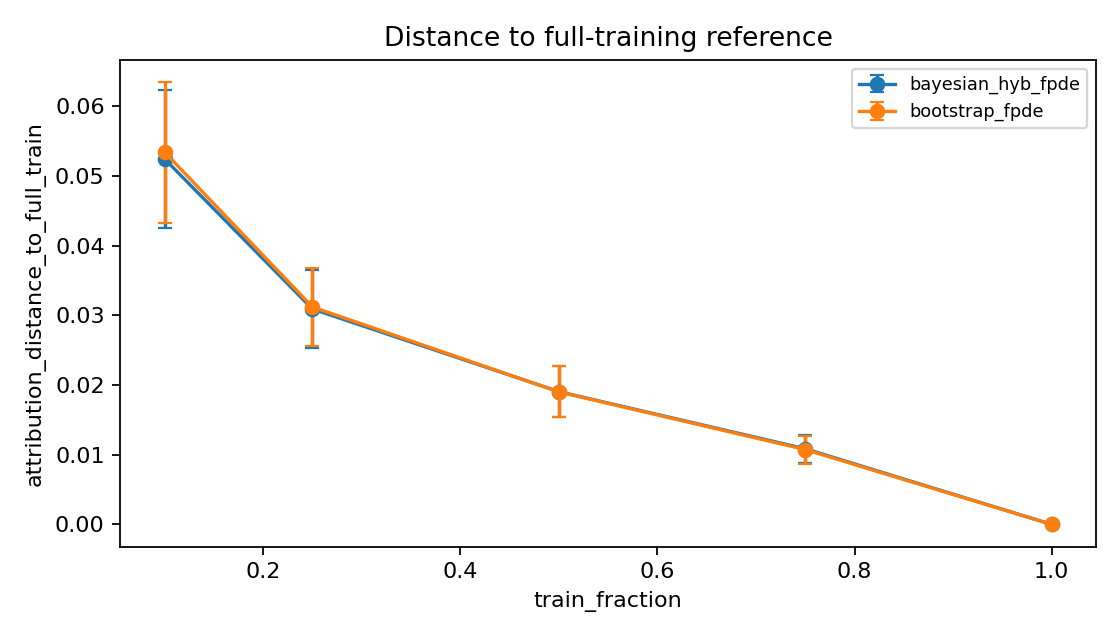
\includegraphics[width=\linewidth]{paper/figures/distance_to_full_train_vs_training_size.png}
\caption{Attribution distance to the full-training empirical reference as a function of training fraction.}
\label{fig:distance_to_full_train_vs_training_size}
\end{figure}

\begin{figure}[t]
\centering
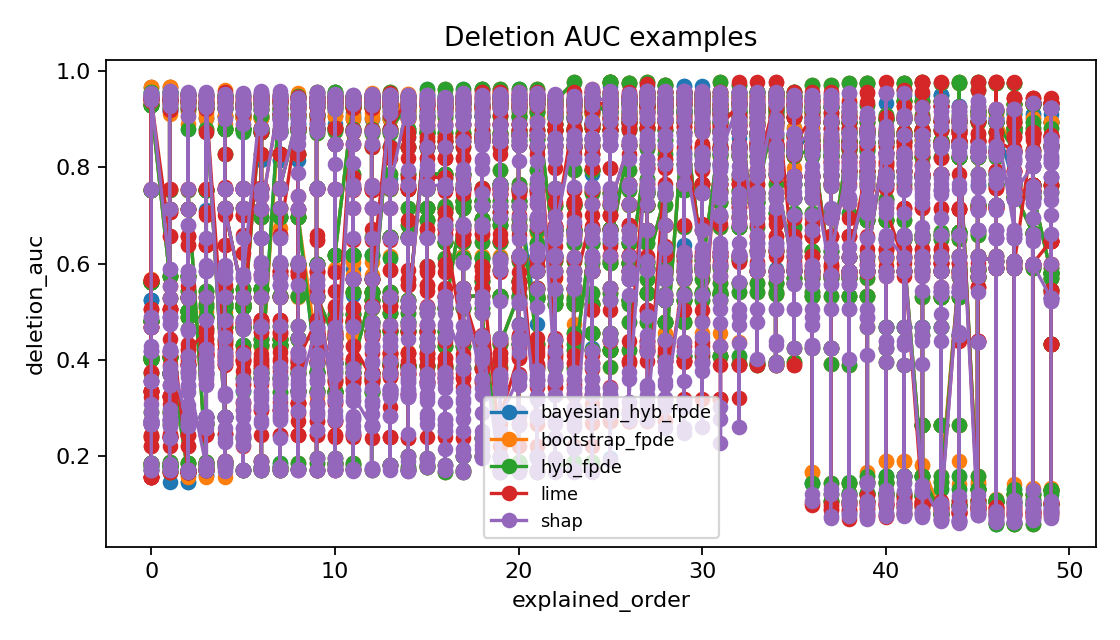
\includegraphics[width=\linewidth]{paper/figures/deletion_curves_examples.png}
\caption{Example deletion curves used as baseline-dependent model-output consistency evidence.}
\label{fig:deletion_curves_examples}
\end{figure}

\begin{figure}[t]
\centering
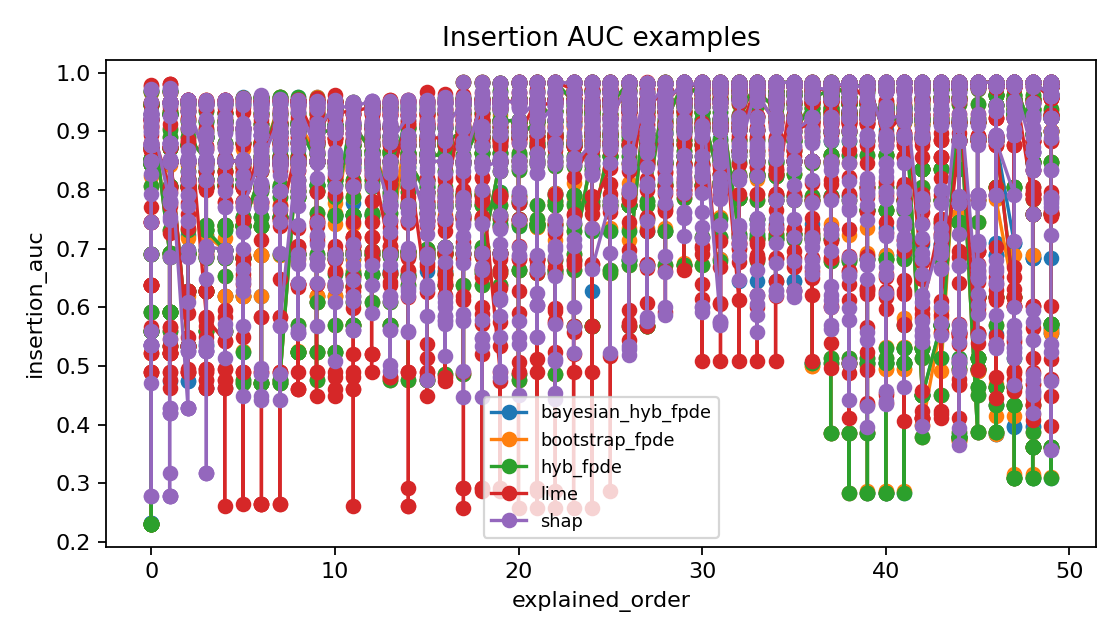
\includegraphics[width=\linewidth]{paper/figures/insertion_curves_examples.png}
\caption{Example insertion curves used as baseline-dependent model-output consistency evidence.}
\label{fig:insertion_curves_examples}
\end{figure}


% Sensitivity analysis narrative, tables, and figures.
\section{Sensitivity Analysis}

\subsection{Sensitivity to Posterior Sample Size}

Table~\ref{tab:posterior_sensitivity} reports the posterior-sample-size sensitivity analysis for posterior\_samples values of 100, 300, and 500 at lambda\_hyb = 0.5. Across this tested range, empirical\_reference\_coverage\_95 remained stable at 0.945, and top-k Jaccard overlap across seeds remained 0.896 after aggregation over the five public benchmark datasets. Mean posterior standard deviation was also stable, ranging from 0.0306 to 0.0308, while mean credible interval width increased slightly from 0.1153 to 0.1197.

These results suggest that the reported empirical reference coverage and top-ranked feature overlap were not sensitive to the posterior sample count within the tested range. Fig.~\ref{fig:posterior_samples_mean_ci_width} shows the corresponding credible-interval-width trend. This conclusion is limited to the evaluated grid of posterior\_samples = \{100, 300, 500\}; it should not be generalized to substantially smaller or larger posterior sample sizes without additional experiments.

\subsection{Sensitivity to the Hyb-FPDE Mixing Weight}

Table~\ref{tab:lambda_sensitivity} reports the sensitivity analysis over lambda\_hyb values of 0.25, 0.50, and 0.75 at posterior\_samples = 500. Varying lambda\_hyb affected posterior standard deviations and credible interval widths: mean posterior standard deviation increased from 0.0223 at lambda\_hyb = 0.25 to 0.0395 at lambda\_hyb = 0.75, and mean credible interval width increased from 0.0867 to 0.1537 over the same range.

Empirical reference coverage and top-ranked feature overlap remained broadly stable across the tested lambda\_hyb values. Mean empirical\_reference\_coverage\_95 ranged from 0.946 to 0.950, and top-k Jaccard overlap across seeds ranged from 0.883 to 0.896. Distance to the default lambda\_hyb = 0.5 setting was symmetric in the aggregate table for 0.25 and 0.75, while top-k Jaccard to the default remained high. Fig.~\ref{fig:lambda_hyb_distance_to_default} visualizes the distance-to-default behavior. These findings are restricted to the tested mixing-weight range and should not be overgeneralized beyond it.

\begin{table}[t]
\centering
\caption{Sensitivity to posterior sample size at lambda\_hyb = 0.5.}
\label{tab:posterior_sensitivity}
\begin{tabular}{r r r r r r}
        \hline
        posterior\_samples & empirical\_reference\_coverage\_95 & Mean posterior std. & Mean CI width & Spearman & Top-k Jaccard \\
        \hline
        100 & 0.945 & 0.0306 & 0.1153 & 0.903 & 0.896 \\
        300 & 0.945 & 0.0308 & 0.1188 & 0.896 & 0.896 \\
        500 & 0.945 & 0.0308 & 0.1197 & 0.900 & 0.896 \\
        \hline
\end{tabular}
\end{table}

\begin{table*}[t]
\centering
\caption{Sensitivity to the Hyb-FPDE mixing weight at posterior\_samples = 500.}
\label{tab:lambda_sensitivity}
\begin{tabular}{r r r r r r r r}
        \hline
        lambda\_hyb & empirical\_reference\_coverage\_95 & Mean posterior std. & Mean CI width & Spearman & Top-k Jaccard & Distance to default & Top-k Jaccard to default \\
        \hline
        0.25 & 0.946 & 0.0223 & 0.0867 & 0.885 & 0.896 & 0.0699 & 1.000 \\
        0.50 & 0.945 & 0.0308 & 0.1197 & 0.900 & 0.896 & 0.0000 & 1.000 \\
        0.75 & 0.950 & 0.0395 & 0.1537 & 0.898 & 0.883 & 0.0699 & 0.993 \\
        \hline
\end{tabular}
\end{table*}

\begin{figure}[t]
\centering
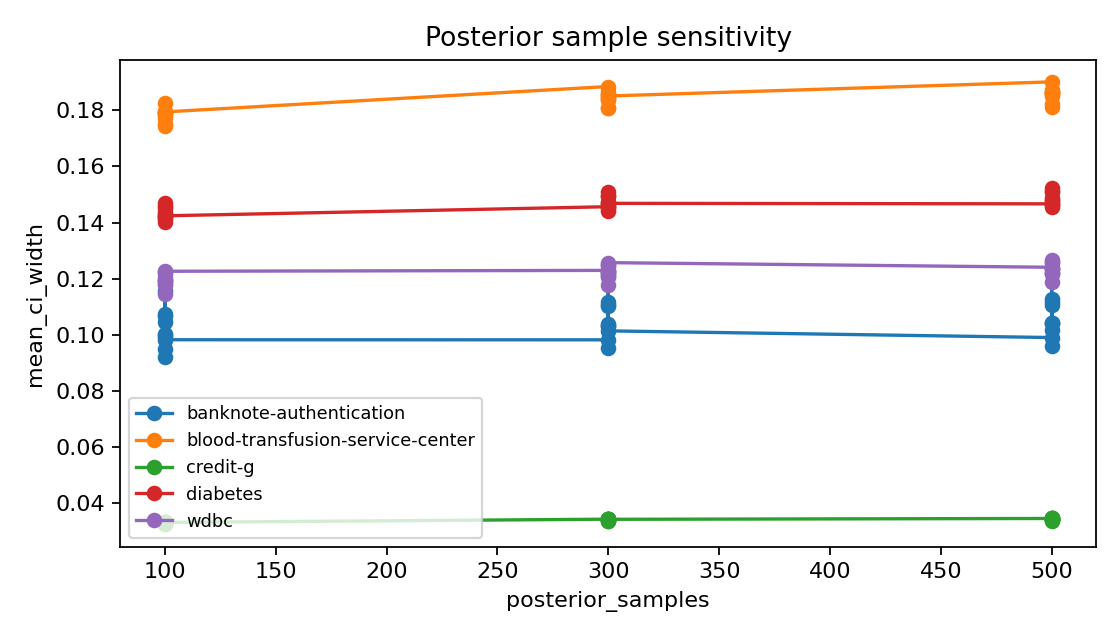
\includegraphics[width=\linewidth]{paper/figures/posterior_samples_mean_ci_width.png}
\caption{Mean credible interval width across the tested posterior sample sizes.}
\label{fig:posterior_samples_mean_ci_width}
\end{figure}

\begin{figure}[t]
\centering
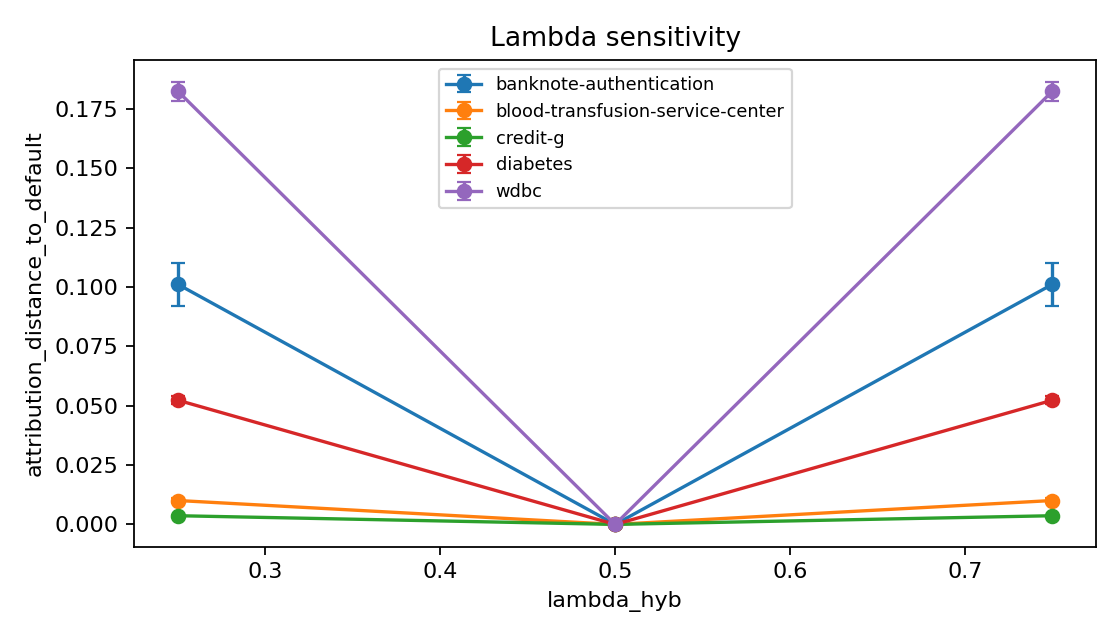
\includegraphics[width=\linewidth]{paper/figures/lambda_hyb_distance_to_default.png}
\caption{Attribution distance to the default lambda\_hyb setting across tested Hyb-FPDE mixing weights.}
\label{fig:lambda_hyb_distance_to_default}
\end{figure}


% Reproducibility artifact narrative and table.
\section{Reproducibility Artifact}

The IEEE Access artifact uses a public-data-only design based on five OpenML benchmark tasks. The main public-data experiment is configured by \texttt{configs/openml\_public\_ieee\_access.yaml}, and the sensitivity analysis is configured by \texttt{configs/openml\_public\_ieee\_access\_sensitivity.yaml}. Table~\ref{tab:reproducibility_artifact} summarizes the artifact components and their paths.

The main results are generated by the GitHub Actions workflow \texttt{.github/workflows/ieee-access-bayesian-fpde-experiments.yml}. The sensitivity results are generated by \texttt{.github/workflows/ieee-access-sensitivity.yml}. The completed main workflow run used run ID 27142484670, and the completed sensitivity workflow run used run ID 27142497585. Both are associated with git commit \texttt{1c24109f3ec412843703174550922b2f8e7ab72a}.

The generated result CSVs are stored under \texttt{results\_ieee/} for the main experiments and \texttt{results\_ieee\_sensitivity/} for the sensitivity analyses. The corresponding figures are stored under \texttt{figures\_ieee/} and \texttt{figures\_ieee\_sensitivity/}, with copied manuscript-ready references under \texttt{paper/figures/}. The workflow logs are stored under \texttt{logs\_ieee/} and \texttt{logs\_ieee\_sensitivity/}.

Manuscript tables in \texttt{paper/tables/} are generated from the completed result CSVs by \texttt{scripts/build\_ieee\_access\_tables.py}; the script does not edit generated result CSVs and does not require internet access. Local smoke or test-mode outputs are intended only for software validation and should not be reported as paper results. The numerical results reported in the manuscript should be taken from the completed corrected \texttt{ieee\_full} and \texttt{sensitivity\_full} artifacts.

\begin{table*}[t]
\centering
\caption{Reproducibility artifact components for the IEEE Access experiments.}
\label{tab:reproducibility_artifact}
\begin{tabular}{l l l}
        \hline
        Component & Path & Purpose \\
        \hline
        Main config & configs/openml\_public\_ieee\_access.yaml & Main public-data experiment configuration \\
        Sensitivity config & configs/openml\_public\_ieee\_access\_sensitivity.yaml & Sensitivity experiment configuration \\
        Main workflow & .github/workflows/ieee-access-bayesian-fpde-experiments.yml & GitHub Actions workflow for main outputs \\
        Sensitivity workflow & .github/workflows/ieee-access-sensitivity.yml & GitHub Actions workflow for sensitivity outputs \\
        Main results & results\_ieee/ & Aggregate CSV outputs for main experiments \\
        Sensitivity results & results\_ieee\_sensitivity/ & Aggregate CSV outputs for sensitivity analyses \\
        Main figures & figures\_ieee/ & Figures generated from main results \\
        Sensitivity figures & figures\_ieee\_sensitivity/ & Figures generated from sensitivity results \\
        Logs & logs\_ieee/, logs\_ieee\_sensitivity/ & Workflow execution logs \\
        \hline
\end{tabular}
\end{table*}

